\subsection{Tutorial zu Gephi}\label{tutorial}

Dieses Kapitel enthält ein kurzes Tutorial zum Arbeiten mit dem Open Source-Programm \textit{Gephi}. Wie bereits erwähnt, sind die Installationsdateien im Unterordner \textit{gephi} enthalten.
\begin{table}[H]
    \begin{center}
        \begin{tabular}{|c|p{7cm}|} 
            \hline  relative\_ausgaenge.gexf  & Unbearbeitetes Netzwerk mit den ersten $100$ Positionen; Gewichtung der Kanten: relative Ausgänge\\
            \hline  relative\_ausgaenge\_pos\_10.gexf  & Unbearbeitetes Netzwerk mit den ersten $10$ Positionen; Gewichtung der Kanten: relative Ausgänge\\
            \hline  relative\_ausgaenge\_pos\_10\_Layout.gephi  & Bearbeitetes Netzwerk mit den ersten $10$ Positionen und Layout; Gewichtung der Kanten: relative Ausgänge\\
            \hline  relative\_eingaenge.gexf  & Unbearbeitetes Netzwerk mit den ersten $100$ Positionen; Gewichtung der Kanten: relative Eingänge\\  
            \hline  relative\_eingaenge\_pos\_10.gexf  & Unbearbeitetes Netzwerk mit den ersten $10$ Positionen; Gewichtung der Kanten: relative Eingänge\\
            \hline relative\_eingaenge\_pos\_10\_Layout.gephi  & Bearbeitetes Netzwerk mit den ersten $10$ Positionen und Layout; Gewichtung der Kanten: relative Eingänge\\     
            \hline
        \end{tabular} 
    \end{center}
    \caption{Übersicht der Gephi Dateien}\label{Gephi_dateien}
\end{table}
\noindent Das Program liest \textit{gexf}-Dateien ein und erstellt daraus ein Netzwerk aus Knoten und Kanten. Die Dateien für dieses Tutorial wurden in \textit{R} mit den Skripten \textit{gexf.R} und \textit{gexf\_support.R} erstellt, die in dem Ornder \textit{r\_scripts} zu finden sind. Mit den Skripten können verschiedene Parameter und Attribute übergeben werden, wie zum Beispiel die farbliche Kodierung der Knoten und die Gewichtung der Kanten. Ein Netzwerk, dass in \textit{Gephi} bearbeitet wurde, kann als \textit{gephi}-Datei abgespeichert werden. Dieses Format kann ausschlieslich in Gephi eingelesen werden. In diesen Dateien sind typischerweise Layouts, das heißt die Anordnung der Knoten, und Filter für die Kanten gespeichert. Tabelle \ref{Gephi_dateien} gibt eine Übersicht über die \textit{gexf}- und \textit{gephi}-Dateien, die im elektronischen Anhang bereits vorhanden sind und mit Hilfe derer das Tutorial beschrieben wird. Für die zwei \textit{gephi}-Dateien wurde der \textit{ForceAtlas2}-Algorithmus angewendet und die Anordnung der Knoten daraufhin noch manuell bearbeitet.\\
Nach der Installation und dem Öffnen des Programms, können über \textit{File $ \rightarrow $ Open}, die Dateien geöffnet werden. Abbildung \ref{workspace} enthält einen Screenshot des Workspaces nach dem Laden von \textit{relative\_ausgaenge.gexf}. Im lilafarbenen Kasten links oben sind die einzelnen Bearbeitungsmodi von \textit{Gephi} auswählbar. \textit{Overview} ist dafür gedacht den Graphen zu bearbeiten und mit einem Layout zu versehen. Im \textit{Data Laboratory} können einzelne Knoten und Kanten bearbeitet und neue Attribute hinzufügt werden. Die \textit{Preview} liefert eine Ansicht der Datei, wie sie im Falle eines Exports aussieht.
\begin{figure}[H]
    \centering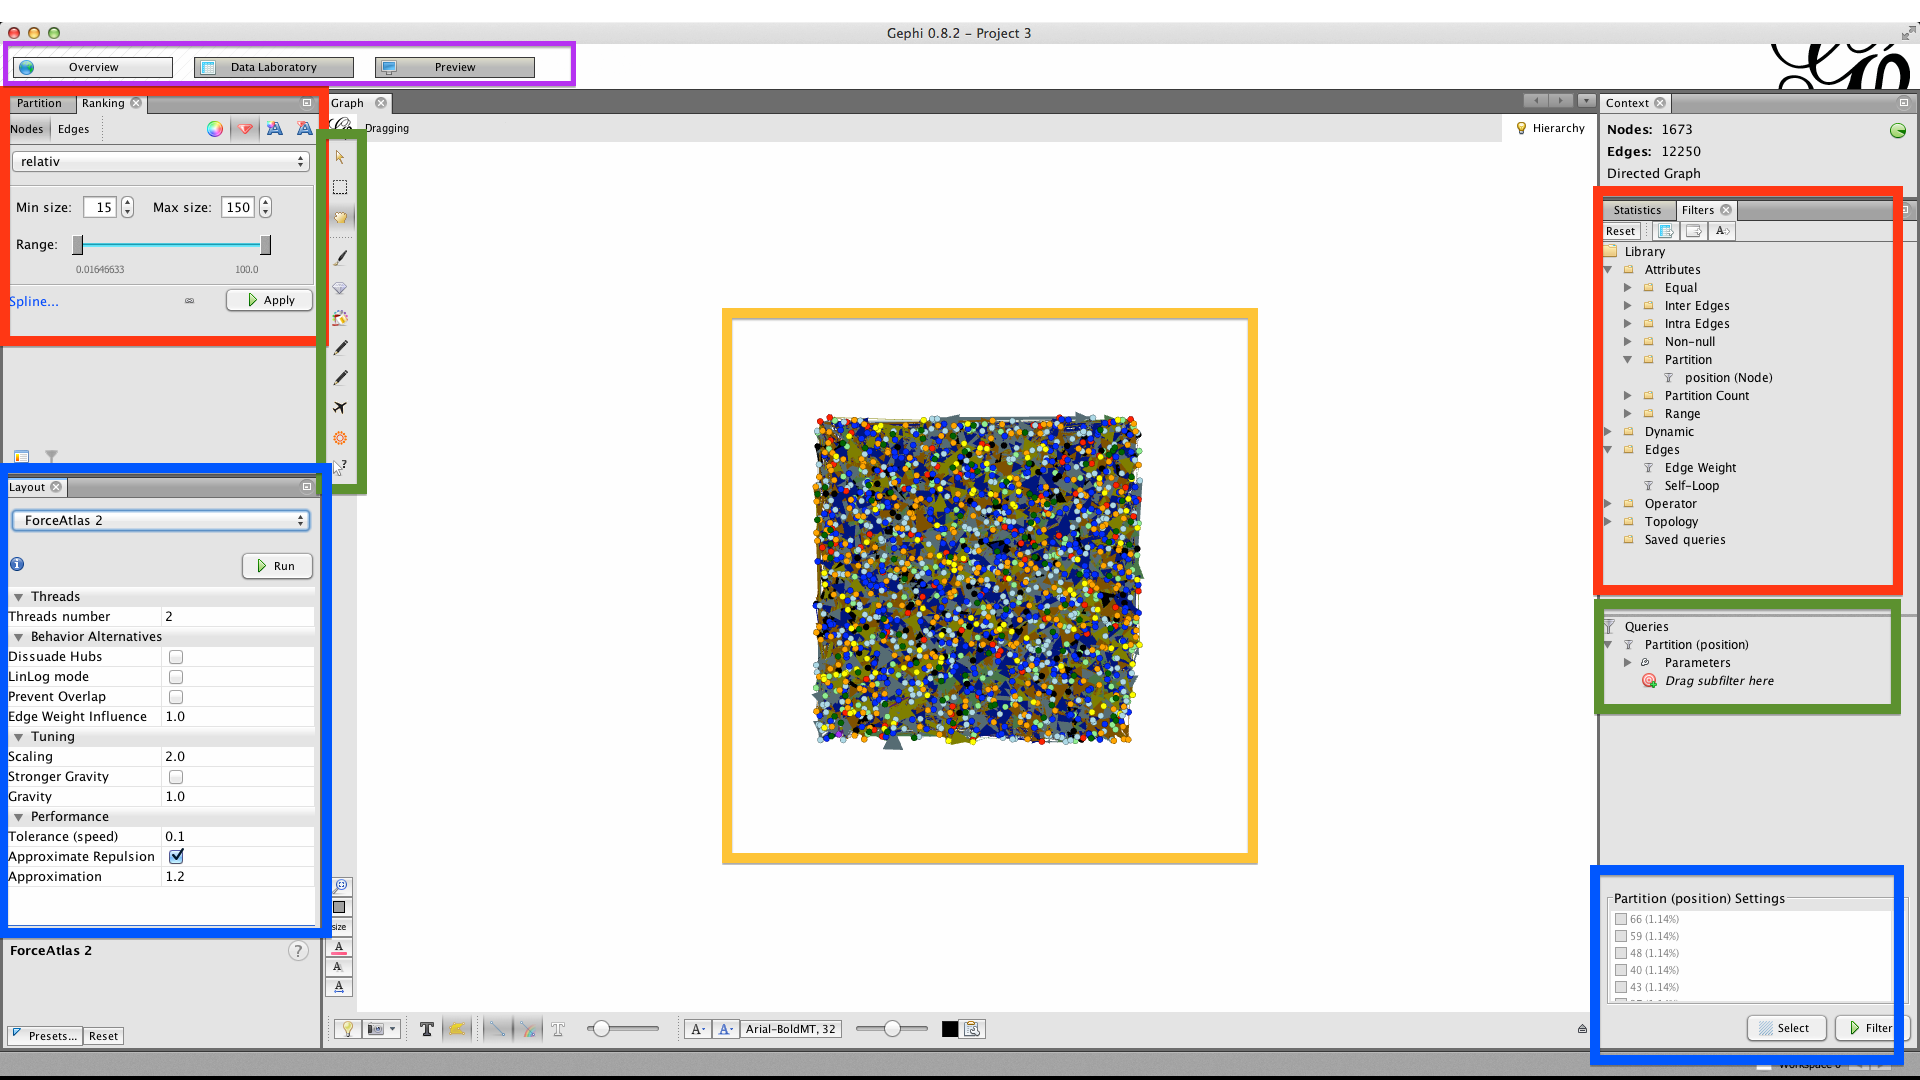
\includegraphics[scale=0.23]{workspace.png}\caption{Workspace in Gephi}\label{workspace}
\end{figure}
\noindent Gelb markiert, in der Mitte der Abbildung, ist das Netzwerk zu sehen. Diese viereckige Struktur besitzt der Graph nach dem Einlesen einer \textit{gexf}-Datei. Anhand der Optionen in dem blauen Kasten auf der linken Seite, kann das Netzwerk bearbeitet werden. Hier kann der gewünschte Algorithmus ausgewählt werden, der die räumliche Anordnung der Knoten berechnet. Zusätzlich können die Parameter des Algorithmus verändert werden. Der Parameter \textit{Edge Weight Influence} steuert den Einfluss der Gewichtung der Kanten auf die Anordnung der Knoten und mit \textit{Scaling} kann die Größe des Graphen festgelegt werden. \textit{Approximate Repulsion} regelt die Konvergenz des Graphen und sollte abgewählt werden, um einen übersichtlicheres Netzwerk zu bekommen. Das Aktivieren von \textit{Prevent Overlap} bewirkt, dass die Knoten nicht überlappen. Durch Klicken auf die Schaltfläche \textit{Run} kann der Algorithmus gestartet und gestoppt werden. Durch das Ausprobieren von verschiedenen Algorithmen mit verschiedenen Einstellungen können schnell gute Ergebnisse erzielt werden.\\
Um das Layout weiter zu verändern, kann in dem linken roten Kasten die Größe der Kanten und Knoten eingestellt werden. Dafür muss der rote Diamant angeklickt und ein Gewichtungsattribut ausgewählt werden, welches in diesem Fall die Variable \textit{relativ}, das heißt die relative Häufigkeit der Knoten in einer Position ist. Im grünen Feld daneben befinden sich die Optionen für die Maus, beispielsweise die Einstellung, dass man Knoten manuell im Graphen bewegen und positionieren kann. Aber auch die letzte Option ist hilfreich, mit der man durch einen Klick auf einen Knoten, dessen Informationen sehen kann.
\begin{figure}[H]
    \centering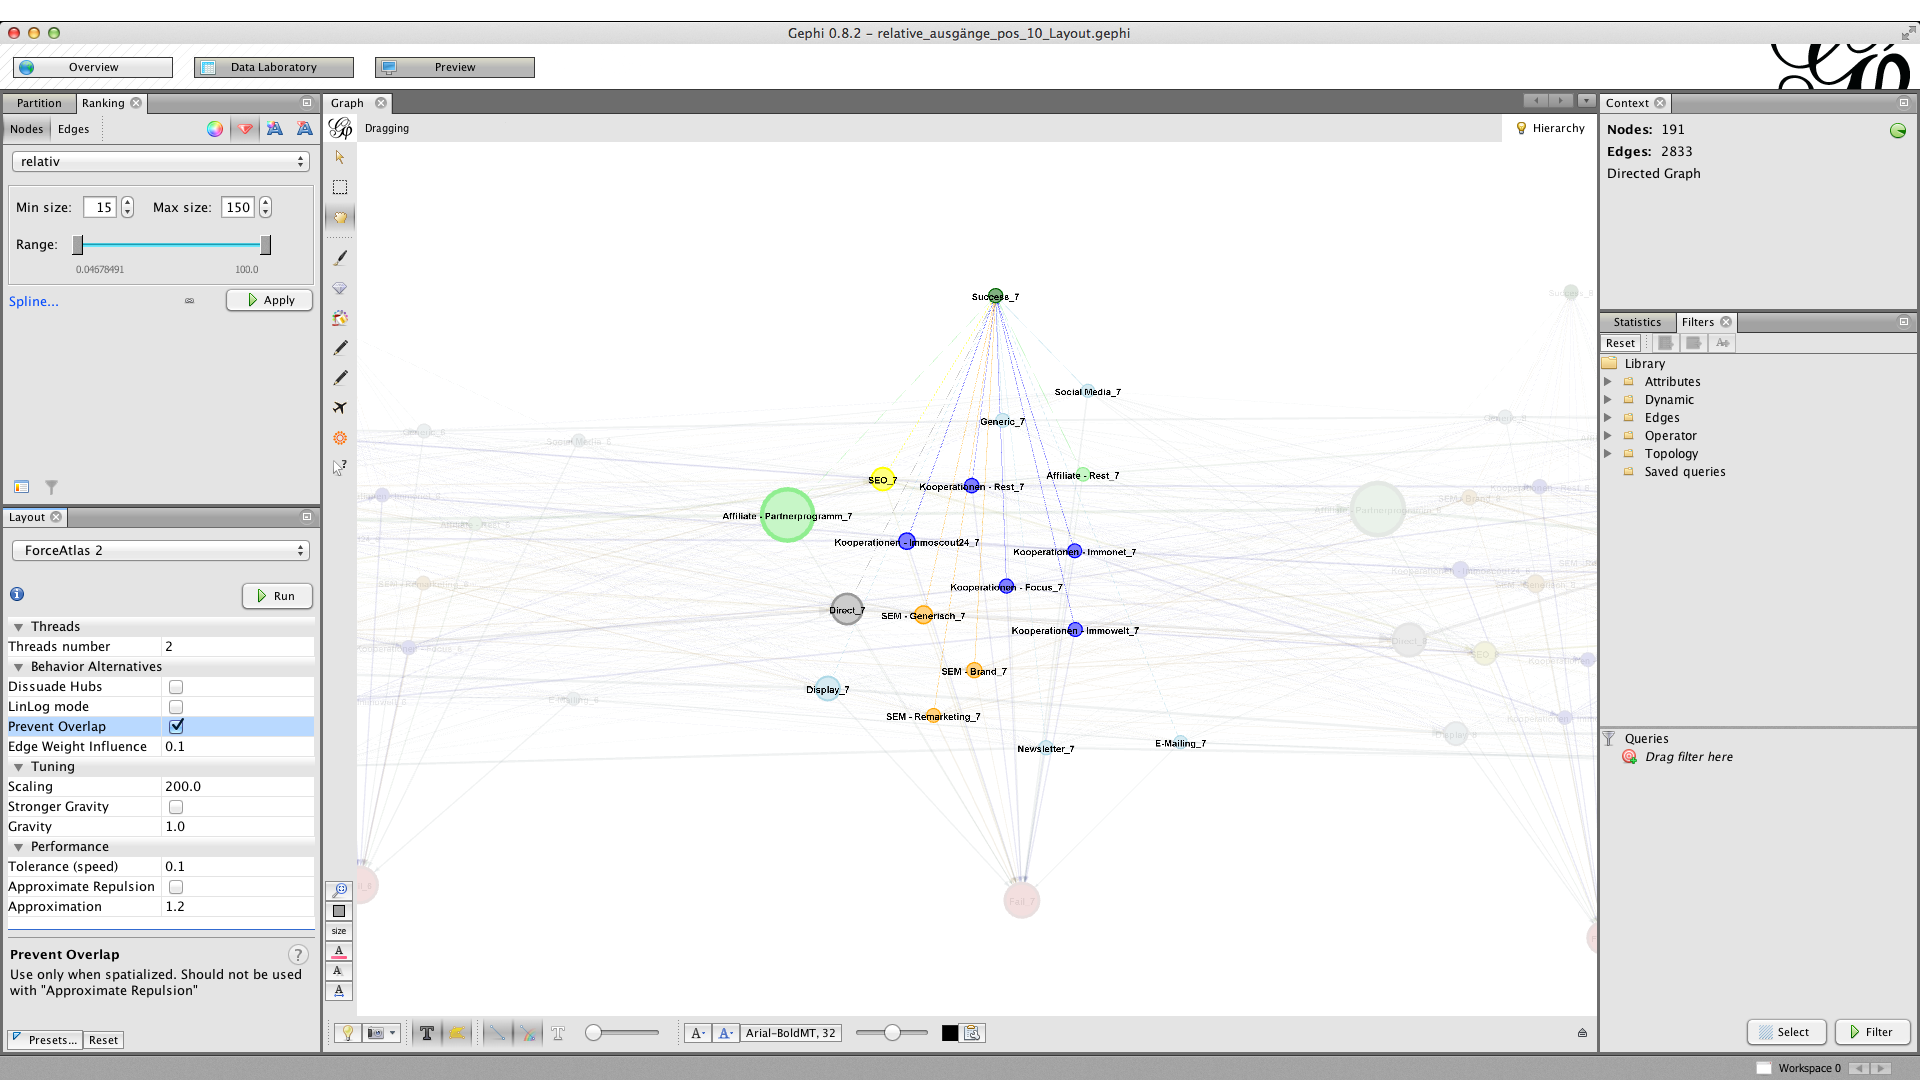
\includegraphics[scale=0.23]{ergebnis_gephi.png}\caption{Nähere Betrachtung einer Position in Gephi}\label{ergebnis}
\end{figure}
\noindent Im roten Feld auf der rechten Seite kann man \textit{Statistics} und \textit{Filters} anwenden. Unter \textit{Filters} kann bezüglich der übergebenen Attribute gefiltert werden. Bei \textit{Partition} befindet sich die Position als Attribut, mit der eingestellt werden kann welche Positionen im Graphen angezeigt werden. Dieser Filter muss in den grünen Kasten gezogen werden, um die Auswahlmöglichkeiten im blauen Kasten zu bekommen. Hier können dann die gewünschten Position ausgewählt werden und mittels dem Button \textit{Filter} aktiviert werden. Desweiteren kann auch einen \textit{subfilter}, also ein zweiter Filter angewendet werden, beispielsweise das \textit{Edge Weight}, das heißt die Gewichtung der Kanten. Generell empfiehlt es sich, den Graphen zunächst zu filtern und dann den Layout Algorithmus anzuwenden, da sich dieser je nach Filterung anpasst. Weitere hilfreiche Features des Programms befinden sich in der Fußzeile des Workspaces, beispielsweise das Ein- oder Ausblenden der Knotenlabels mithilfe des großen \textit{T} oder die Screenshot Funktion.\\
Um das Netzwerk näher zu analysieren, kann durch Scrollen in den Graphen gezoomt und durch Halten der rechten Maustaste und gleichzeitiges Bewegen der Maus navigiert werden. Durch das Bewegen das Mauszeigers auf einen Knoten, werden außerdem alle Knoten, die mit eben diesem verbunden sind, hervorgehoben. In Abbildung \ref{ergebnis} ist dies an Position $7$ dargestellt. Hier wurde der Knoten \textit{Success\_7} angewählt und es ist zu erkennen, dass dieser Knoten mit allen Kampagnen der siebten Position verbunden ist. Durch die Anwendung eines Filters für die Kanten, fallen einige dieser Verbindungen weg und es können interessante Ergebnisse erzielt werden.\\
Um ein bearbeitetes Netzwerk als Bilddatei abzuspeichern, muss es exportiert werden. Dafür muss man links oben den Reiter \textit{Preview} auswählen. Nützliche Einstellungen beim Export sind im lilafarbenen Feld in Abbildung \ref{export} zu finden. \textit{Rescale Weight} sorgt dafür, dass die Kanten nicht zu dick sind und das Abwählen von \textit{Curved} macht das Netzwerk übersichtlicher. Um Änderungen sichtbar zu machen, muss der Button \textit{Refresh} in der grünen Box angeklickt werden. Außerdem kann der Graph hier dann als \textit{SVG}-, \textit{PDF}- oder \textit{PNG}-Datei abgespeichert werden.
\begin{figure}[H]
    \centering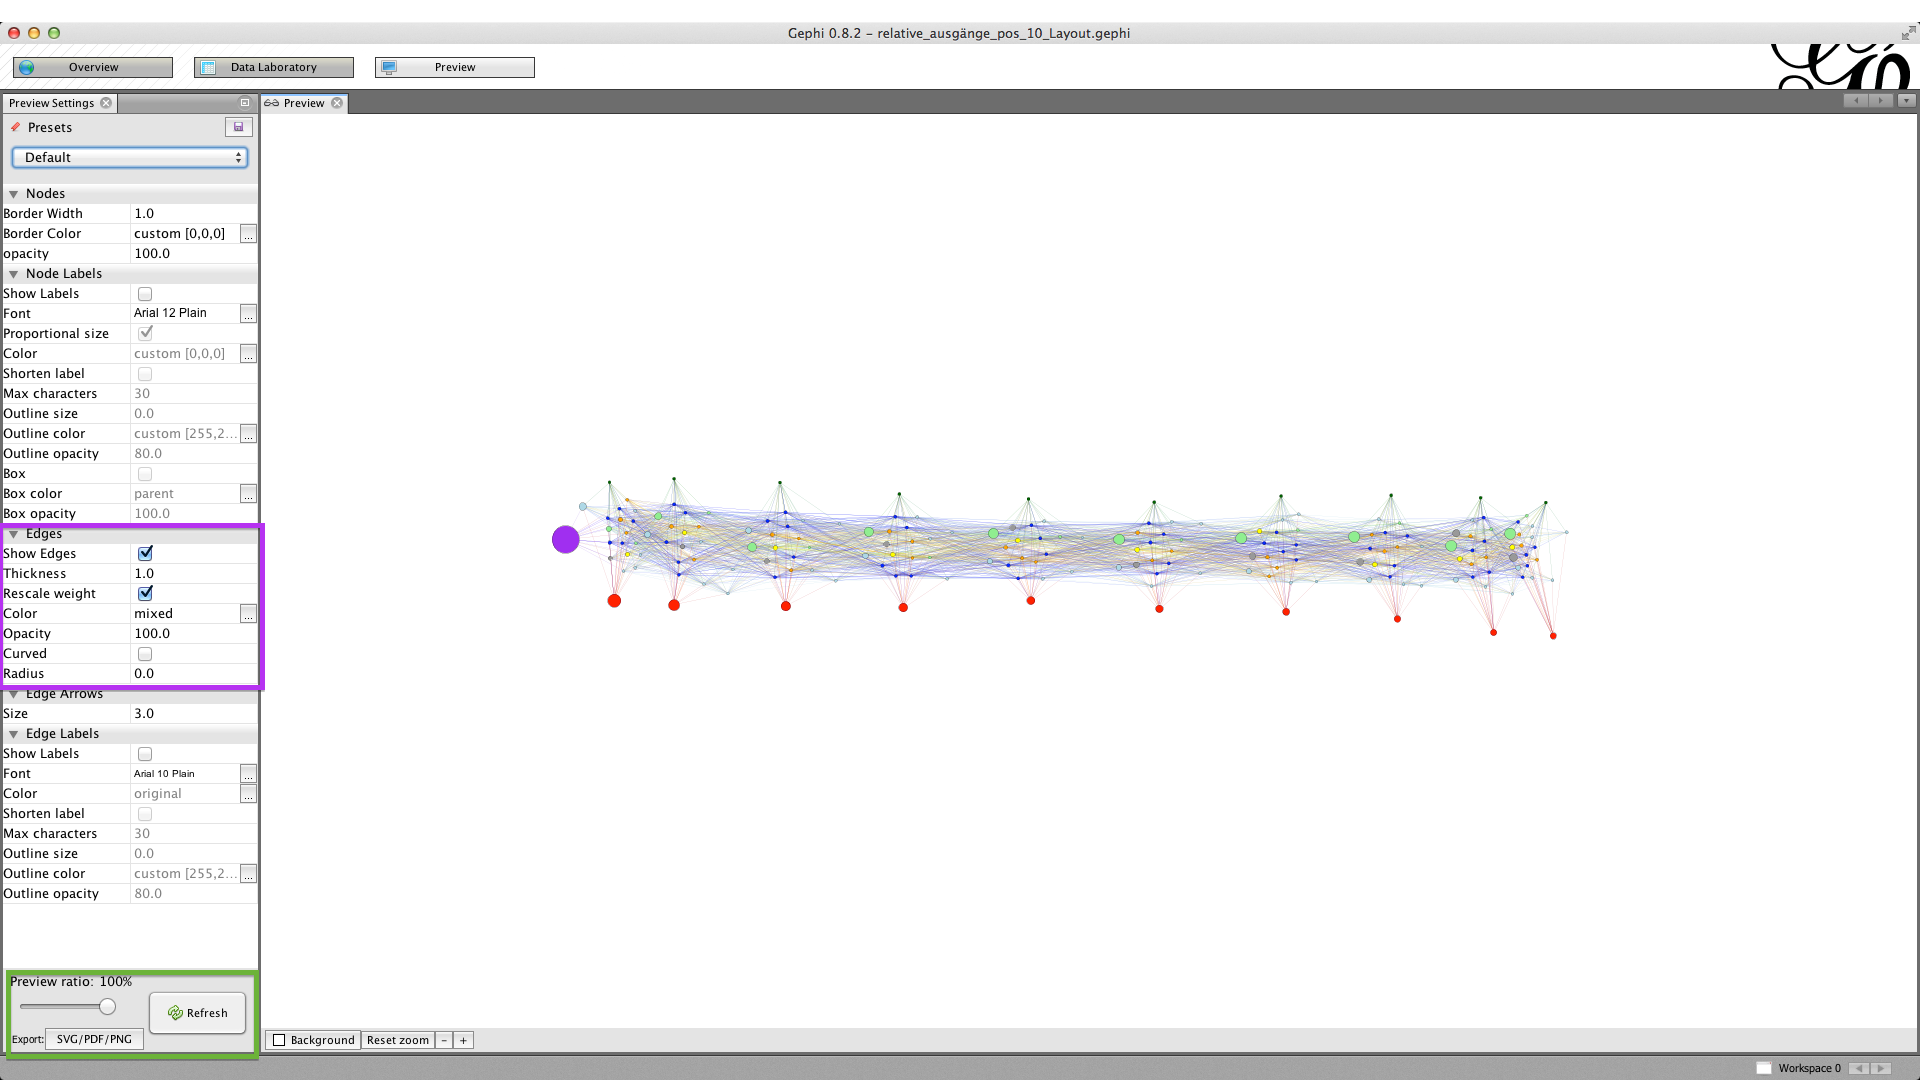
\includegraphics[scale=0.23]{Preview.png}\caption{Export in Gephi}\label{export}
\end{figure}
